\documentclass[conference,10pt]{IEEEtran}

\usepackage{amsmath,amssymb,amsfonts}
\usepackage{graphicx}
\usepackage{booktabs}
\usepackage{cite}
\usepackage{xcolor}
\usepackage{placeins}
\usepackage{hyperref}

\hypersetup{colorlinks=true,linkcolor=blue,citecolor=blue,urlcolor=blue}
\graphicspath{{../../figures/hyqad/}}
\renewcommand{\arraystretch}{1.12}
\newtheorem{proposition}{Proposition}

\title{Calibrated and Kernel-Based Detection of QKD\\Implementation Attacks: A Controlled Simulation Study}

\author{
  \IEEEauthorblockN{Arnav Kapoor}
  \IEEEauthorblockA{Department of Computer Science\\
  \textit{IISER Bhopal}\\
  Bhopal, India\\
  arnavkapoor23@iiserb.ac.in}
}

\begin{document}

\maketitle

\begin{abstract}
Machine-learning detectors for quantum key distribution (QKD) implementation
attacks are usually evaluated on simulated telemetry, and frequently report
near-perfect accuracy. We show that such numbers can be an artifact of the
simulator: without operating-condition drift, a single telemetry feature
separates attacks from normal blocks perfectly. We build a seeded decoy-state
BB84 telemetry simulator with drift in loss, misalignment, detector efficiency
and background light, finite-size QBER noise, and a single \emph{attack-strength}
parameter $s$ that scales four attack signatures (photon-number splitting,
detector blinding, Trojan horse, intercept-resend) from blatant to subtle. On it
we compare a Laplace Gaussian-process classifier (GP), an amplitude-encoding
fidelity-kernel SVM (AE-SVM, 3 qubits, computed exactly and verified against a
PennyLane circuit to $10^{-14}$), RBF-SVM, random forests and a GP+AE-SVM
stacking model, all at matched training sizes over 10 seeds. At $s=0.3$, every
supervised model lands between $0.80$ and $0.84$ MCC; random forest is best or
tied-best throughout, and the GP is neither the most accurate nor the best
calibrated (ECE $0.047$ vs.\ $0.030$ for isotonic-calibrated RF), so it is not
the best basis for uncertainty-based deferral. The amplitude kernel does carry
a usable inductive bias: it wins on direction-only control tasks and, on
unseen attack types, matches RBF-SVM---but only because one feature (a
Mahalanobis distance) carries the input's magnitude. Removing that feature
drops AE-SVM's zero-day AUC from $0.95$ to $0.55$, while appending a constant
``norm anchor'' coordinate before encoding restores it to $0.94$. Code, data and
every result file are released.
\end{abstract}

\begin{IEEEkeywords}
Quantum key distribution, anomaly detection, Gaussian processes, quantum kernels, calibration, simulation methodology
\end{IEEEkeywords}

\section{Introduction}
\label{sec:intro}

QKD derives its security from physics~\cite{bennett1984quantum,gisin2002quantum},
but deployed systems leak through implementation side channels: photon-number
splitting (PNS) against multi-photon pulses~\cite{huttner1995photon,lutkenhaus2002pns},
detector control by bright illumination~\cite{makarov2006effects,lydersen2010hacking},
Trojan-horse probing of the transmitter or receiver~\cite{gisin2006trojan,jain2014trojan},
and intercept-resend~\cite{bennett1992experimental}. Decoy states~\cite{lo2005decoy}
and measurement-device-independent designs~\cite{lo2012measurement} close some of
these channels; continuous telemetry monitoring is a complementary defense, and
machine learning has been applied to it~\cite{mao2020detecting} and to related
QKD control problems~\cite{ren2021machine}.

Two methodological problems make it hard to know what such detectors are worth.
First, they are typically trained and tested on simulated telemetry, and a
simulator in which normal operation sits at one fixed operating point makes
almost any attack signature separable. Second, ``quantum'' components are often
evaluated at very different training sizes from classical baselines, so a
comparison confounds model and data.

This paper is a controlled simulation study that addresses both. Our
contributions are:
\begin{enumerate}
\item A seeded decoy-state BB84 telemetry simulator with operating drift and an
  explicit attack-strength axis $s$, together with leakage checks. Without drift,
  a single feature gives perfect separation; with it, detection degrades smoothly
  from MCC $\approx 0.97$ at $s=1$ to $\approx 0.5$ at $s=0.05$ (Section~\ref{sec:sim}).
\item A matched-$n$ comparison of a GP, an exact amplitude-encoding fidelity
  kernel, RBF-SVM, random forest (RF) and stacking at every training size from
  $25$ to $1400$ (Section~\ref{sec:results}).
\item A mechanism for when the amplitude kernel generalizes to unseen attacks,
  confirmed by ablation: it needs a feature that carries the input's magnitude,
  which can be supplied by a one-line norm anchor (Section~\ref{sec:zeroday}).
\item A calibration and selective-prediction comparison showing that the GP's
  posterior is not the best uncertainty signal on this data
  (Section~\ref{sec:calib}).
\end{enumerate}
All results are from simulation; Section~\ref{sec:limits} states what this does
and does not establish.

\section{Related Work}
\label{sec:related}

Hardware countermeasures monitor detector statistics directly, for example
after-pulse and efficiency estimates computed in real time~\cite{dasilva2012monitoring}.
Mao et al.~\cite{mao2020detecting} trained neural networks to recognise attacks on
continuous-variable QKD from measured statistics. We study discrete-variable
decoy-state BB84 telemetry and focus on evaluation methodology, calibrated
uncertainty and kernel inductive bias rather than on a new detector.

Quantum kernel methods embed data in a Hilbert space through a state-preparation
circuit and use state overlaps as a kernel~\cite{havlicek2019supervised,schuld2021machine}.
Provable advantages exist for specially constructed problems~\cite{liu2021rigorous},
and whether a quantum kernel helps on a given dataset depends on how its
geometry matches the data~\cite{huang2021power}. Amplitude encoding is a case in
which the overlap is classically computable (Proposition~\ref{prop:exact}), so it
isolates the kernel's inductive bias from any question of quantum speed-up.
Gaussian processes~\cite{rasmussen2006gaussian} and other Bayesian
methods~\cite{perusquia2022bayesian} provide model-based uncertainty for anomaly
detection; post-hoc recalibration~\cite{platt1999probabilistic,zadrozny2002transforming,guo2017calibration}
is the standard alternative for point-estimate models.

\section{Telemetry Simulator}
\label{sec:sim}

\subsection{Channel model}
Each sample is one key-generation block of a decoy-state BB84 link over $L=50$\,km
of fiber ($\alpha=0.2$\,dB/km). For mean photon number $\mu \sim \mathcal{U}(0.1,1)$,
transmittance $T=10^{-A/10}$ and detector efficiency $\eta$, the gain and QBER of a
Poisson source are~\cite{lo2005decoy}
\begin{align}
Q_\mu &= Y_0 + \bigl(1-e^{-\eta T\mu}\bigr)(1+p_{\mathrm{ap}}),\\
E_\mu &= \bigl[\tfrac12 Y_0 + e_d\,(1-e^{-\eta T\mu})(1+p_{\mathrm{ap}})\bigr]/Q_\mu ,
\end{align}
with afterpulse probability $p_{\mathrm{ap}}=0.005$. Normal operation is not a
single point: per block, the attenuation $A$ drifts by $\mathcal{N}(0,0.3^2)$\,dB
around $\alpha L$, $\eta$ by $3\%$ around $0.9$, and the misalignment error $e_d$,
dark-count probability $Y_0$ and background rate are log-normal around $0.01$,
$10^{-5}$ and $100$\,s$^{-1}$ (log-scale s.d.\ $0.4$, $0.3$, $0.3$). The two
reported error rates (sifted QBER and decoy-basis error rate) carry independent
finite-size noise $\sqrt{E(1-E)/N_b}$ with $N_b=5000$. Seven measurements are
reported per block: QBER, photon count rate, detection efficiency, dark-count
rate, error rate, attenuation and background rate.

\subsection{Attack models and strength}
The four attacks perturb these measurements as in prior qualitative
descriptions~\cite{huttner1995photon,makarov2006effects,gisin2006trojan,bennett1992experimental}:
PNS removes a fraction $0.3$ of photons and raises QBER by $\mathcal{U}(0.02,0.08)$;
blinding divides efficiency by $1+1.5\gamma$, $\gamma\sim\mathcal{U}(0.5,1.5)$, and
raises QBER by $\mathcal{U}(0.05,0.25)$; Trojan-horse probing multiplies background
by $1+10\rho$, $\rho\sim0.05\,\mathcal{U}(0.5,2)$; intercept-resend raises QBER by
$\mathcal{U}(0.10,0.35)$ and lowers the count rate. These magnitudes are modeling
assumptions, not measured values. Every deviation from the clean block is
multiplied by a strength $s\ge0$, so $s=1$ is the default and $s\to0$ makes an
attack indistinguishable from normal operation (Fig.~\ref{fig:qber}).

\begin{figure*}[t]
  \centering
  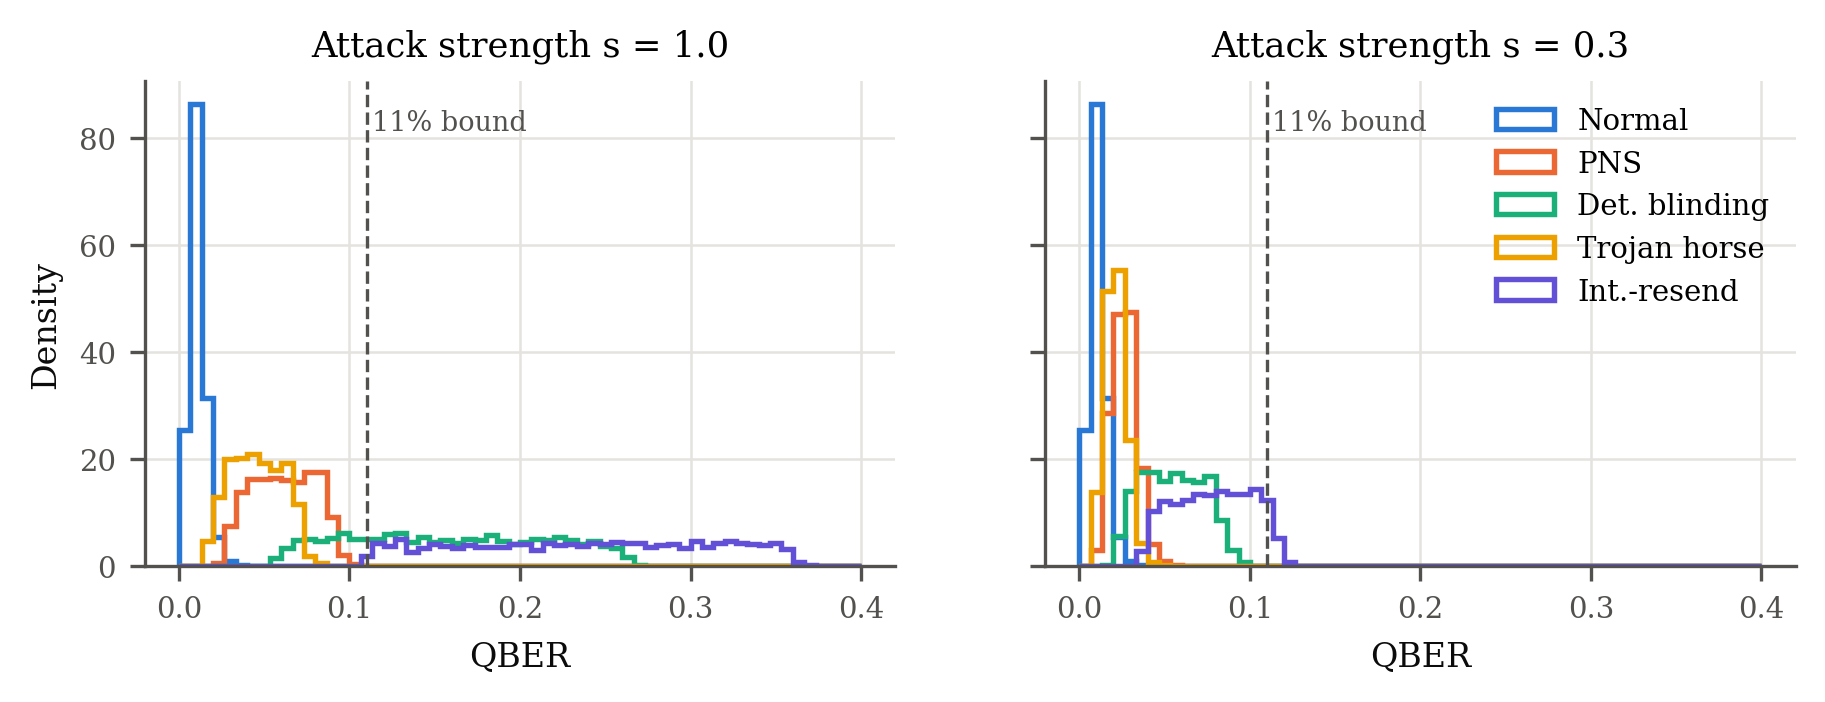
\includegraphics[width=0.92\textwidth]{fig2_qber_dist.png}
  \caption{QBER by class at attack strength $s=1$ and $s=0.3$. At $s=0.3$, PNS and
  Trojan-horse blocks sit well below the 11\% bound and overlap normal operation.}
  \label{fig:qber}
\end{figure*}

\subsection{Leakage checks}
Two properties are tested in the released test suite. (i) Different seeds give
different datasets, and every random draw, including attack perturbations,
derives from the dataset seed. (ii) No single feature is a label proxy: block
timestamps are drawn independently of the label, and a depth-2 decision tree on
any single feature stays below perfect accuracy. We include these checks because
an earlier version of our own pipeline failed both, which made every detector
look near-perfect; we expect the same failure in other simulation-only QKD
detection results.

\section{Detectors and Protocol}
\label{sec:method}

\begin{figure*}[t]
  \centering
  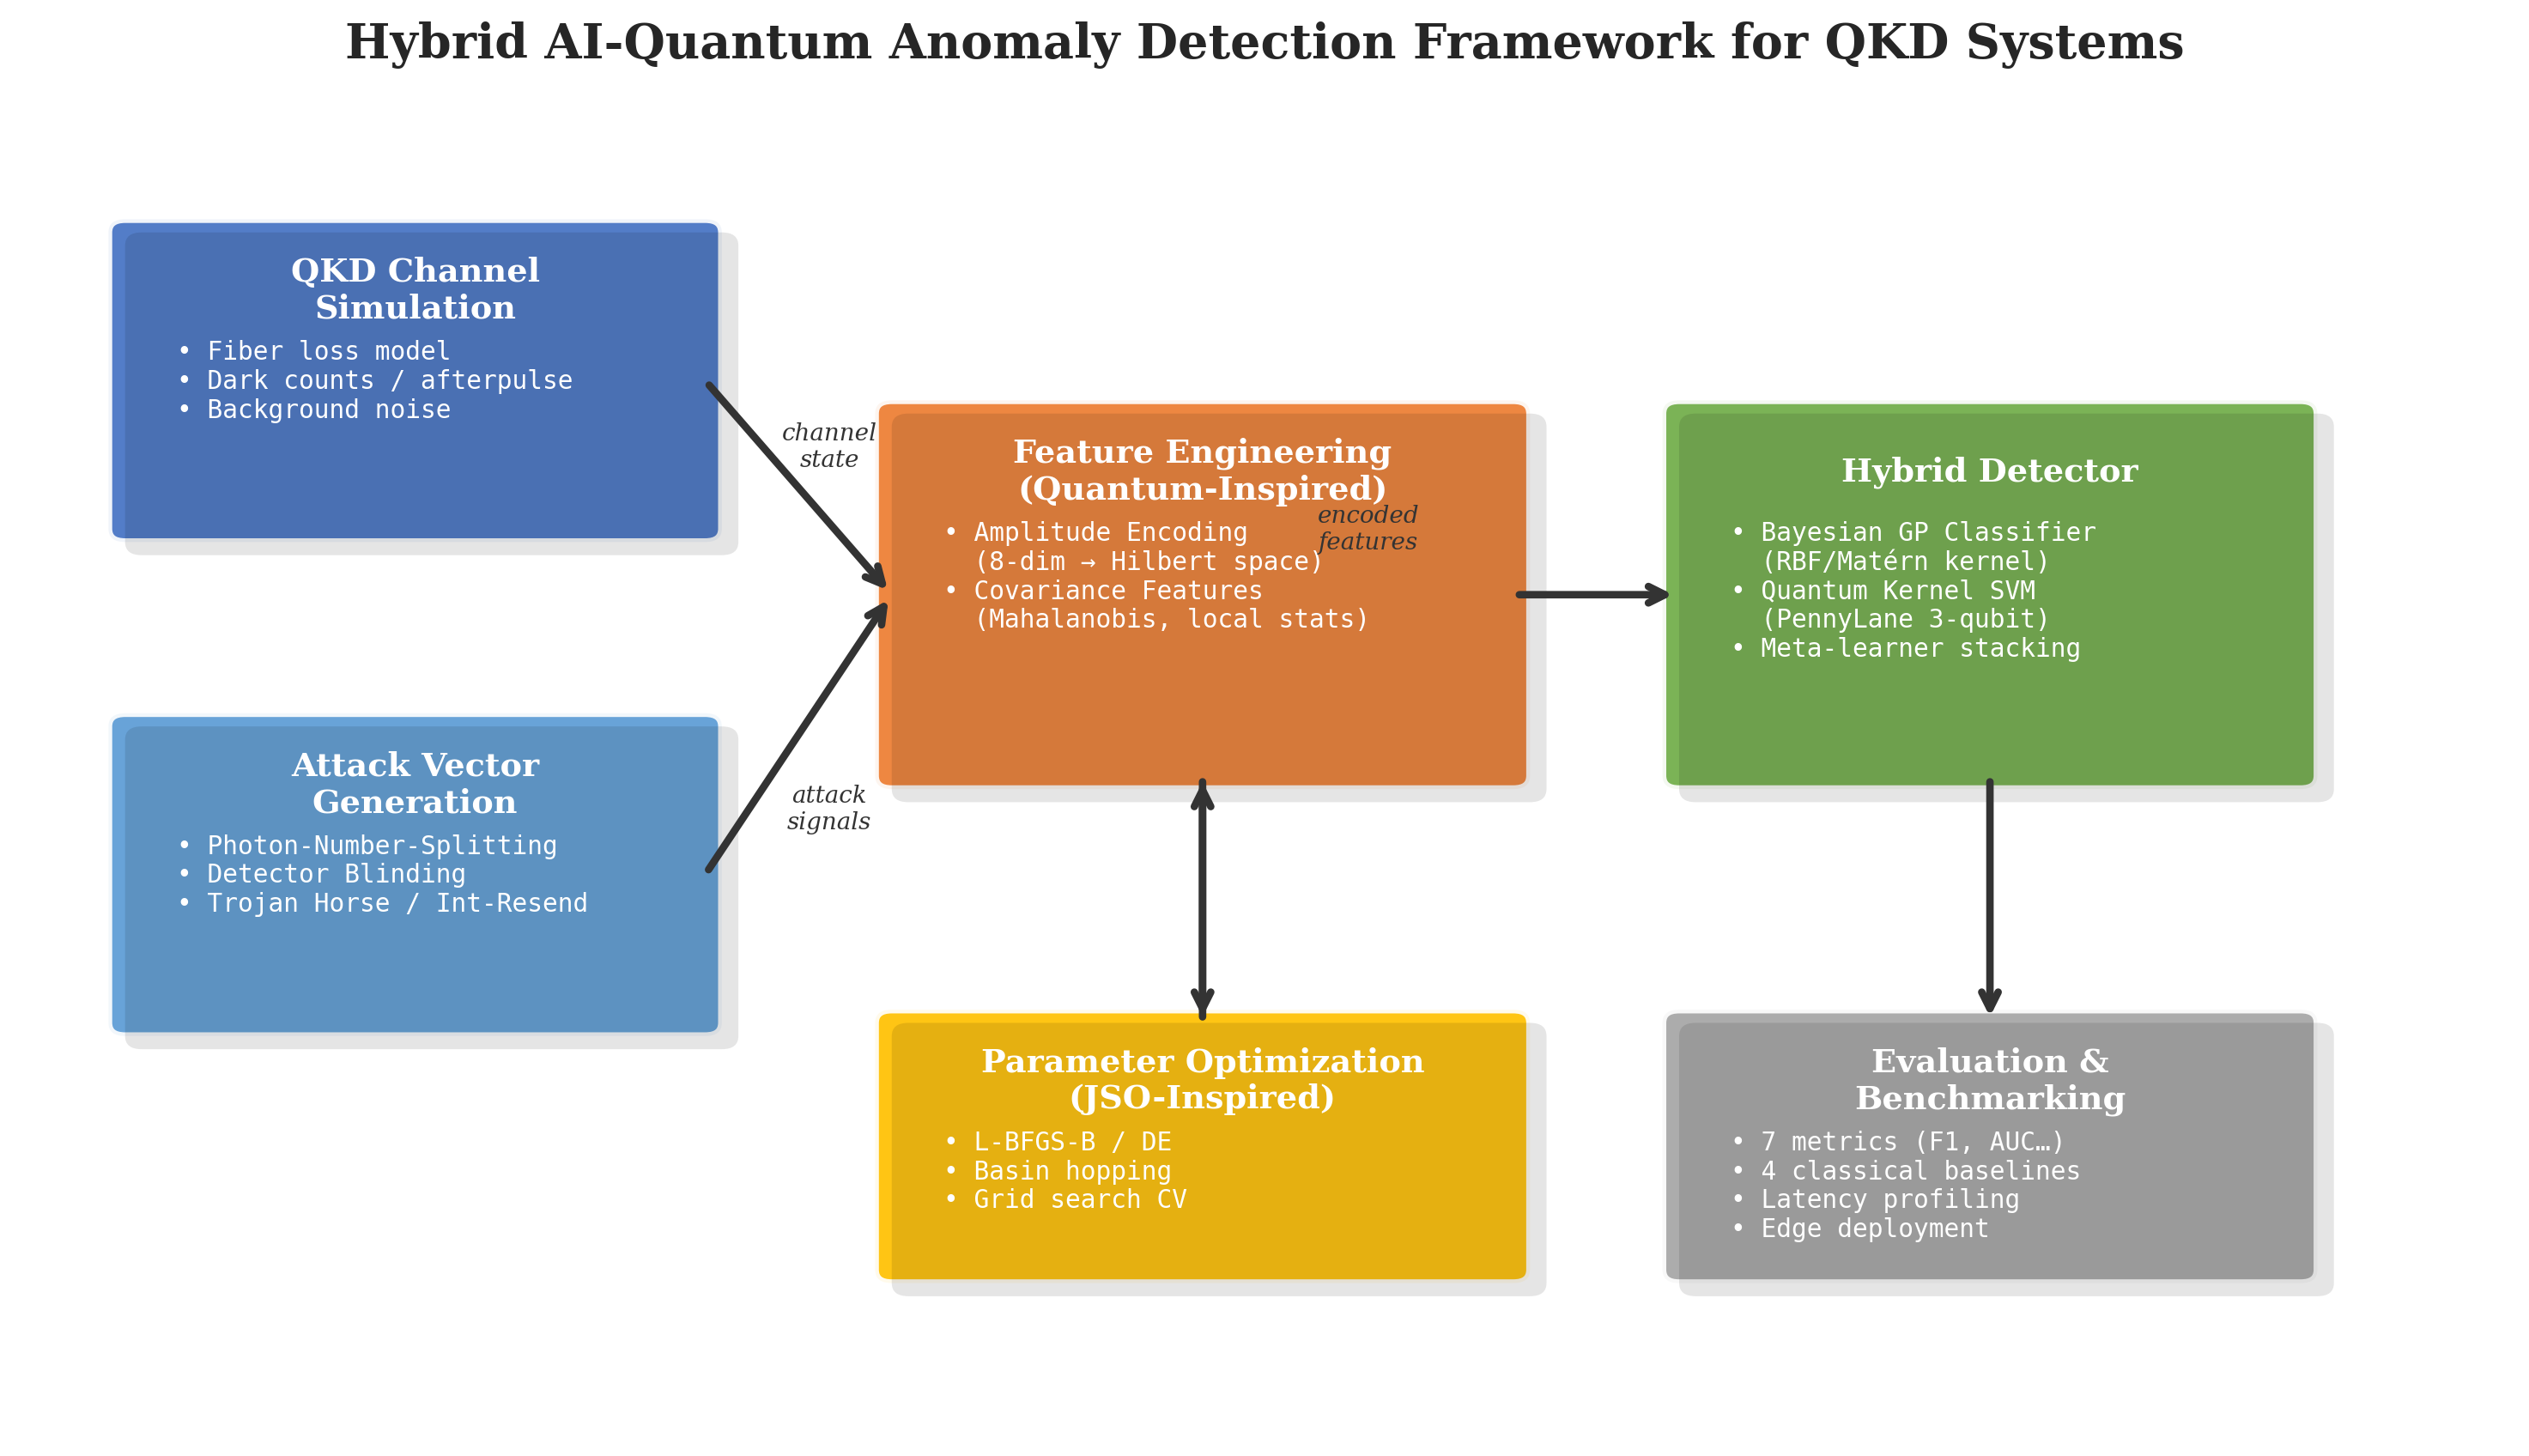
\includegraphics[width=\textwidth]{fig1_framework_hyqad.png}
  \caption{Study design: simulator, attack models with strength $s$, a fixed 8-dimensional feature map shared by every detector, and the evaluation suite.}
  \label{fig:framework}
\end{figure*}

\textbf{Features.} Every detector sees the same 8 features
(Fig.~\ref{fig:framework}): the 7 measurements standardized on the training
split, plus the robust Mahalanobis distance~\cite{rousseeuw1999fast} of the
standardized vector to the training-split normal blocks.

\textbf{Amplitude-encoding fidelity kernel (AE-SVM).} A vector
$\mathbf{x}\in\mathbb{R}^d$ is zero-padded to $2^q$ entries, $q=\lceil\log_2 d\rceil$,
and normalized, giving the state $|\psi(\mathbf{x})\rangle=\sum_i \hat{x}_i|i\rangle$.
The fidelity kernel is $K_A(\mathbf{x},\mathbf{y})=|\langle\psi(\mathbf{x})|\psi(\mathbf{y})\rangle|^2$.

\begin{proposition}\label{prop:exact}
$K_A(\mathbf{x},\mathbf{y}) = (\hat{\mathbf{x}}^{\mathsf{T}}\hat{\mathbf{y}})^2$,
the squared cosine similarity of the inputs. It is computable classically in
$\mathcal{O}(d)$ time per pair and is invariant to $\mathbf{x}\mapsto c\,\mathbf{x}$
for every $c\neq0$, including $c=-1$.
\end{proposition}
\noindent The proof is immediate from real amplitudes and zero padding. We
therefore evaluate the kernel exactly with all 8 features on 3 qubits, and
confirm that a PennyLane~\cite{bergholm2018pennylane} state-vector simulation of
the overlap circuit agrees to $7\times10^{-15}$; the circuit costs $26$\,ms per
kernel entry versus $3\times10^{-4}$\,ms in closed form. The SVM uses $C=1$, balanced
class weights and Platt-scaled probabilities~\cite{platt1999probabilistic}.

\textbf{Baselines.} A Laplace GP classifier~\cite{rasmussen2006gaussian} with an
RBF+white-noise kernel (hyperparameters chosen by marginal likelihood on a
stratified 300-sample subset, then fixed for the full fit); RBF-SVM with the same
SVM settings as AE-SVM; RF (200 trees)~\cite{breiman2001random}, raw and
isotonic-calibrated~\cite{zadrozny2002transforming}; a stacking model (Hybrid)
combining GP and AE-SVM through logistic regression with 3-fold
cross-validation~\cite{wolpert1992stacked}; and three novelty detectors fit on
normal training blocks only (one-class SVM, isolation forest, LOF).

\textbf{Protocol.} $N=2000$ blocks with 30\% attacks (balanced across types),
70/30 stratified split, 10 seeds; we report means with 95\% confidence intervals
over seeds. Matched-$n$ experiments train \emph{every} model on the same
stratified subsample, for $n\in\{25,50,100,200,500,1000,1400\}$. Paired model
comparisons use the exact McNemar test per seed. Zero-day experiments train on
three attack types and test on normal blocks plus the held-out fourth, at
$1{,}200$ test blocks per split.

\section{Results}
\label{sec:results}

\subsection{In-distribution detection}

\begin{table}[t]
  \centering
  \caption{Detection at $n=1400$ (mean $\pm$ 95\% CI, 10 seeds). ECE uses 15 equal-width bins.}
  \label{tab:bench}
  \scriptsize
  \setlength{\tabcolsep}{2.6pt}
  \begin{tabular}{lcccccc}
    \toprule
    & \multicolumn{3}{c}{$s=1.0$} & \multicolumn{3}{c}{$s=0.3$} \\
    \cmidrule(lr){2-4}\cmidrule(lr){5-7}
    Model & MCC & AUC & ECE & MCC & AUC & ECE \\
    \midrule
    RF          & $\mathbf{.975}{\scriptstyle\pm.008}$ & $.999$ & $.013$ & $\mathbf{.834}{\scriptstyle\pm.013}$ & $.969$ & $.030$ \\
    RF-isotonic & $.972{\scriptstyle\pm.008}$ & $.997$ & $\mathbf{.010}$ & $\mathbf{.837}{\scriptstyle\pm.013}$ & $.967$ & $\mathbf{.030}$ \\
    Hybrid      & $.971{\scriptstyle\pm.005}$ & $.999$ & $.015$ & $\mathbf{.833}{\scriptstyle\pm.016}$ & $.969$ & $.037$ \\
    RBF-SVM     & $.969{\scriptstyle\pm.008}$ & $.999$ & $.011$ & $.810{\scriptstyle\pm.015}$ & $.957$ & $.040$ \\
    GP          & $.964{\scriptstyle\pm.009}$ & $.999$ & $.039$ & $.801{\scriptstyle\pm.016}$ & $.956$ & $.047$ \\
    AE-SVM      & $.955{\scriptstyle\pm.011}$ & $.999$ & $.015$ & $.814{\scriptstyle\pm.023}$ & $\mathbf{.970}$ & $.032$ \\
    \midrule
    OC-SVM      & $.838{\scriptstyle\pm.016}$ & $.994$ & -- & $.657{\scriptstyle\pm.017}$ & $.839$ & -- \\
    IF          & $.837{\scriptstyle\pm.021}$ & $.997$ & -- & $.722{\scriptstyle\pm.019}$ & $.929$ & -- \\
    LOF         & $.824{\scriptstyle\pm.021}$ & $.997$ & -- & $.691{\scriptstyle\pm.011}$ & $.924$ & -- \\
    \bottomrule
  \end{tabular}
\end{table}

Table~\ref{tab:bench} reports detection at the full training size. At $s=1$
every supervised model exceeds $0.95$ MCC and $0.99$ AUC, so this operating point
does not discriminate between methods; the novelty detectors, which never see an
attack label, reach $0.82$--$0.84$ MCC. At $s=0.3$ the supervised models spread
between $0.80$ and $0.84$ MCC: RF, isotonic RF and Hybrid lead, and the GP has the
lowest attack recall ($0.78\pm0.02$, against $0.85$ for RF and $0.90$ for
AE-SVM) because it trades recall for specificity ($0.98$). Hybrid improves on
the GP alone (pooled over seeds, Hybrid corrects $154$ GP errors and introduces
$76$; McNemar $p<0.05$ on 4 of 10 seeds) but does not improve on RF. AE-SVM
matches RBF-SVM in accuracy (both $0.920$; McNemar $p>0.05$ on every seed) and has
the highest AUC ($0.970$).

\subsection{Matched training size}

\begin{figure*}[t]
  \centering
  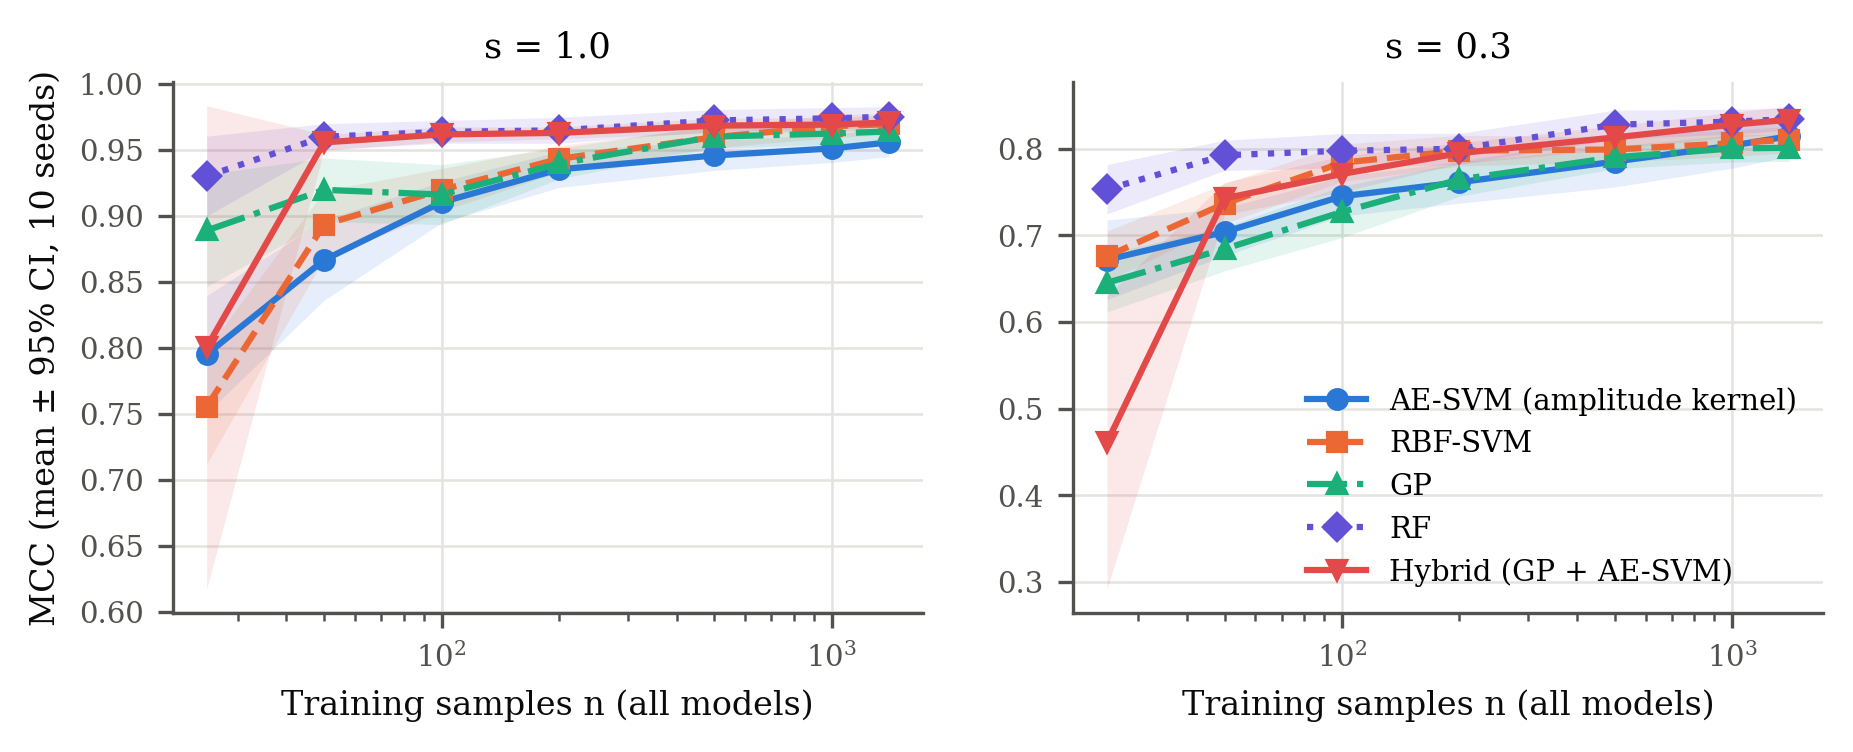
\includegraphics[width=0.92\textwidth]{fig3_matched_n.png}
  \caption{MCC versus training size, every model trained on the same stratified subsample (mean $\pm$ 95\% CI, 10 seeds). The Hybrid model is unstable at $n=25$, where its 3-fold stacking has only $\approx$8 training blocks per fold.}
  \label{fig:matched}
\end{figure*}

Fig.~\ref{fig:matched} trains every model at every $n$. RF is the most
sample-efficient model at both strengths (MCC $0.75$ at $n=25$, $s=0.3$, against
$0.65$--$0.68$ for the kernel methods and GP). The amplitude kernel needs more data
than the RBF kernel to reach the same MCC: at $s=0.3$ AE-SVM trails RBF-SVM by
$0.03$--$0.04$ for $n=50$--$200$ and reaches parity only from $n=1000$
($0.804$ vs.\ $0.806$); at $s=1$ it trails by $0.008$--$0.017$ at every $n\ge50$.
There is no training size at which it is reliably ahead.

\subsection{Attack strength}

\begin{figure*}[t]
  \centering
  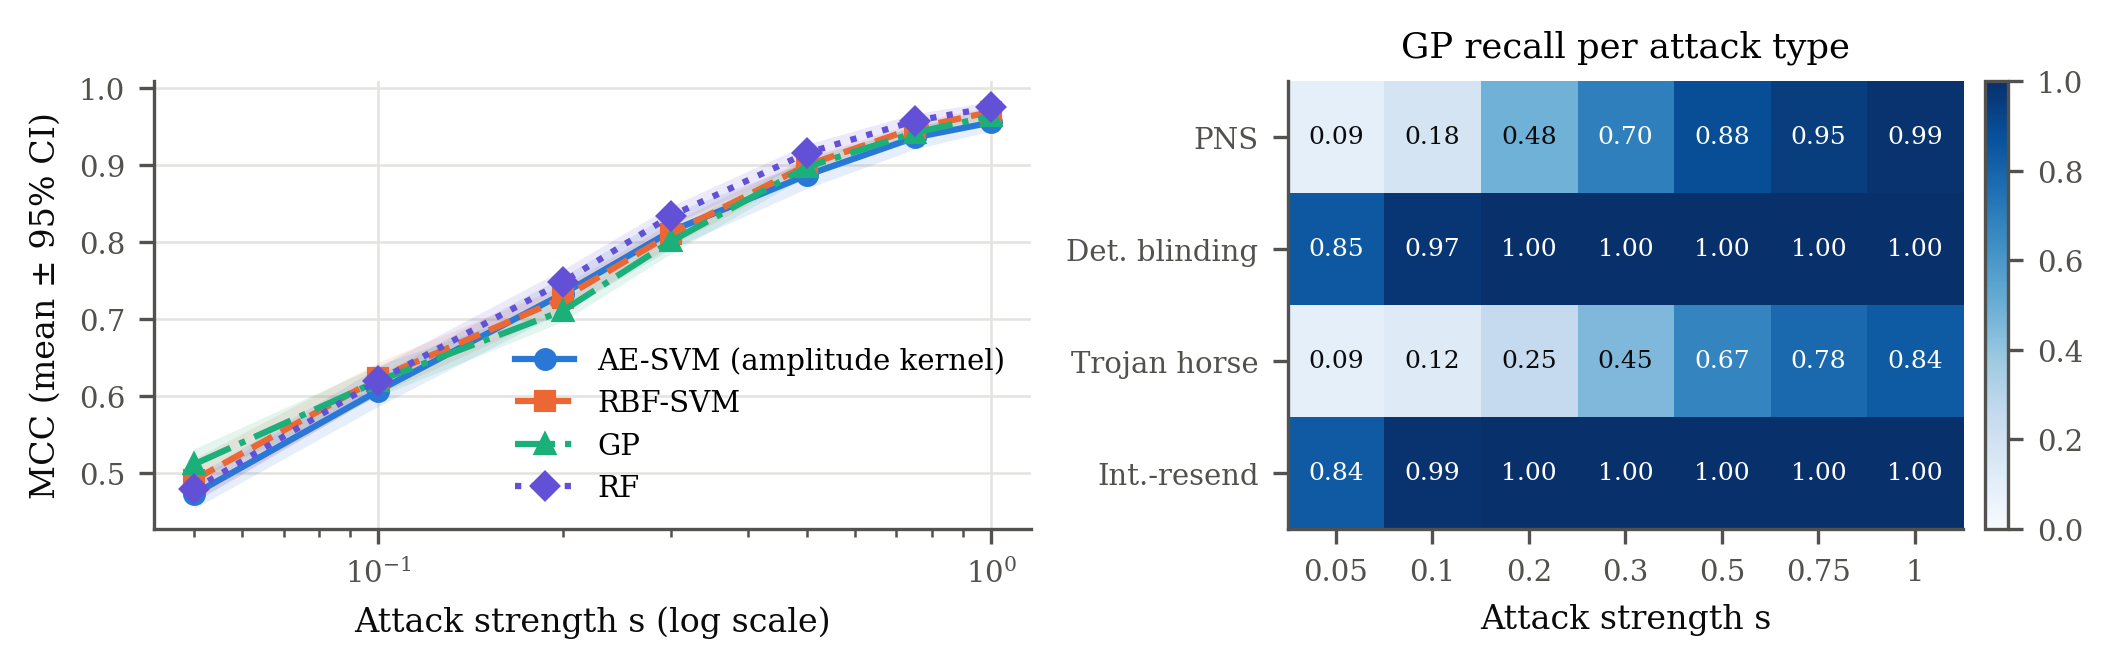
\includegraphics[width=0.92\textwidth]{fig4_strength_sweep.png}
  \caption{Left: MCC versus attack strength at $n=1400$. Right: GP recall per attack type. Trojan-horse and PNS signatures are lost first.}
  \label{fig:strength}
\end{figure*}

All four detectors degrade together as $s$ falls (Fig.~\ref{fig:strength}),
from MCC $0.96$--$0.98$ at $s=1$ to $0.61$--$0.62$ at $s=0.1$ and $0.47$--$0.51$ at
$s=0.05$. RF is best at every $s\ge0.2$; below that all four are within $0.04$
MCC of each other. Per attack type, intercept-resend and detector blinding keep
GP recall $\ge0.97$ down to $s=0.1$ because they move QBER the most, while PNS
and Trojan-horse probing are lost first (Trojan-horse recall $0.45$ at $s=0.3$).

\subsection{Unseen attack types}
\label{sec:zeroday}

\begin{figure*}[t]
  \centering
  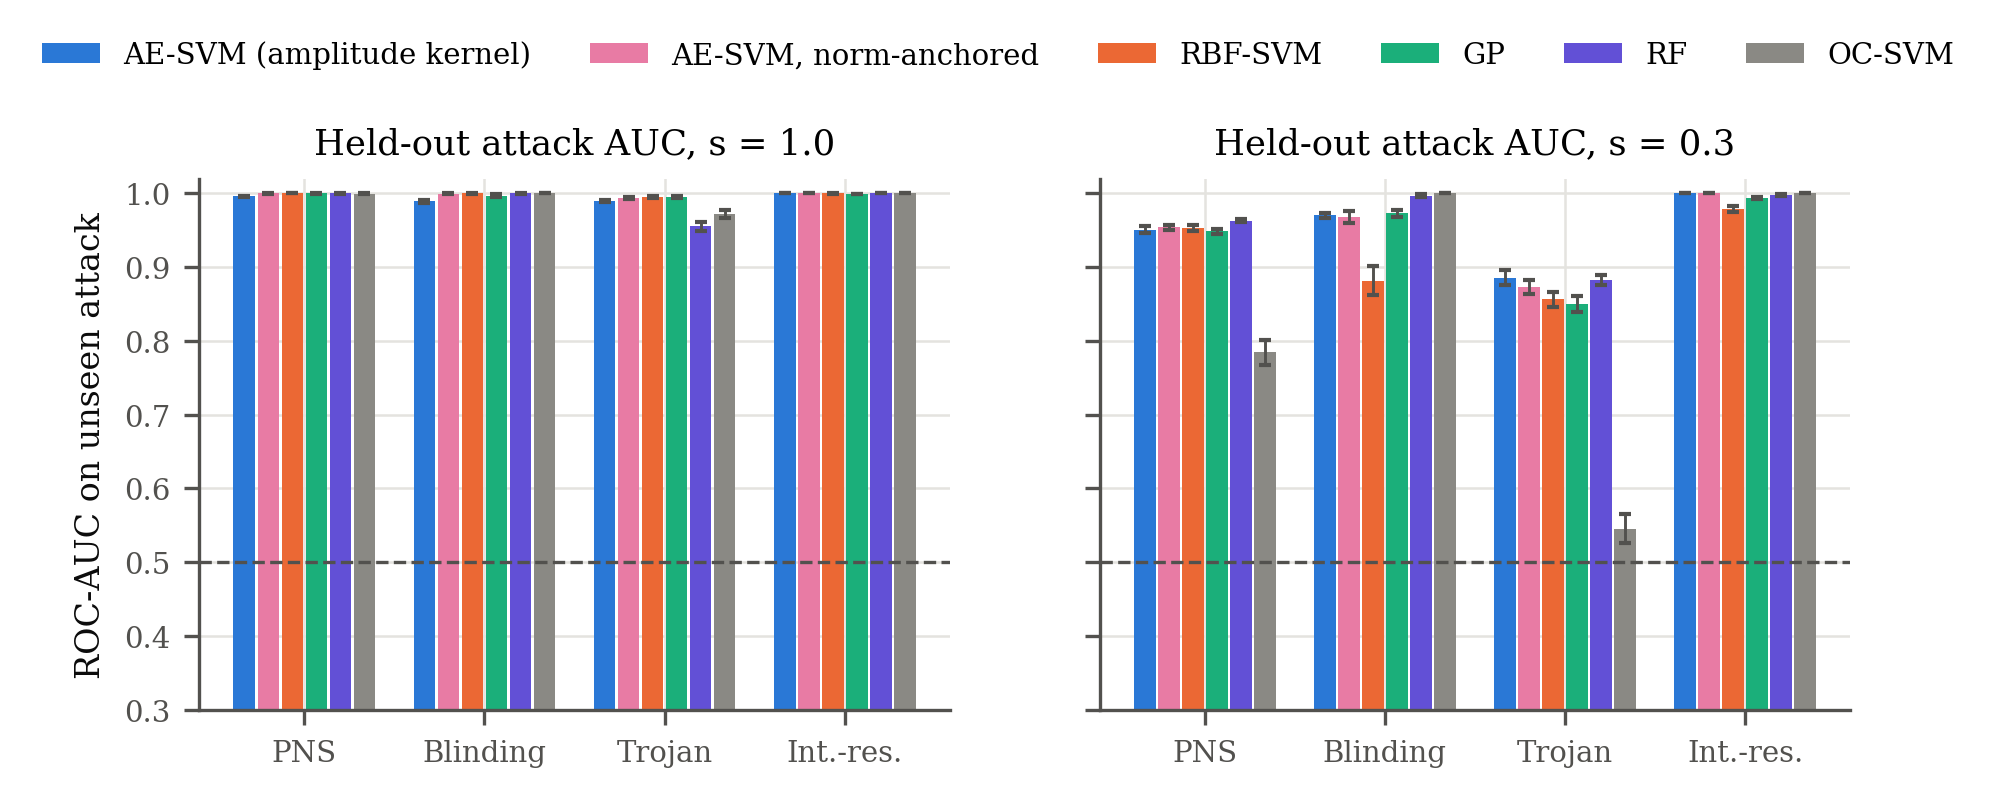
\includegraphics[width=0.92\textwidth]{fig5_zeroday.png}
  \caption{AUC on a held-out attack type, training on the other three (mean $\pm$ 95\% CI, 10 seeds).}
  \label{fig:zeroday}
\end{figure*}

\begin{figure}[t]
  \centering
  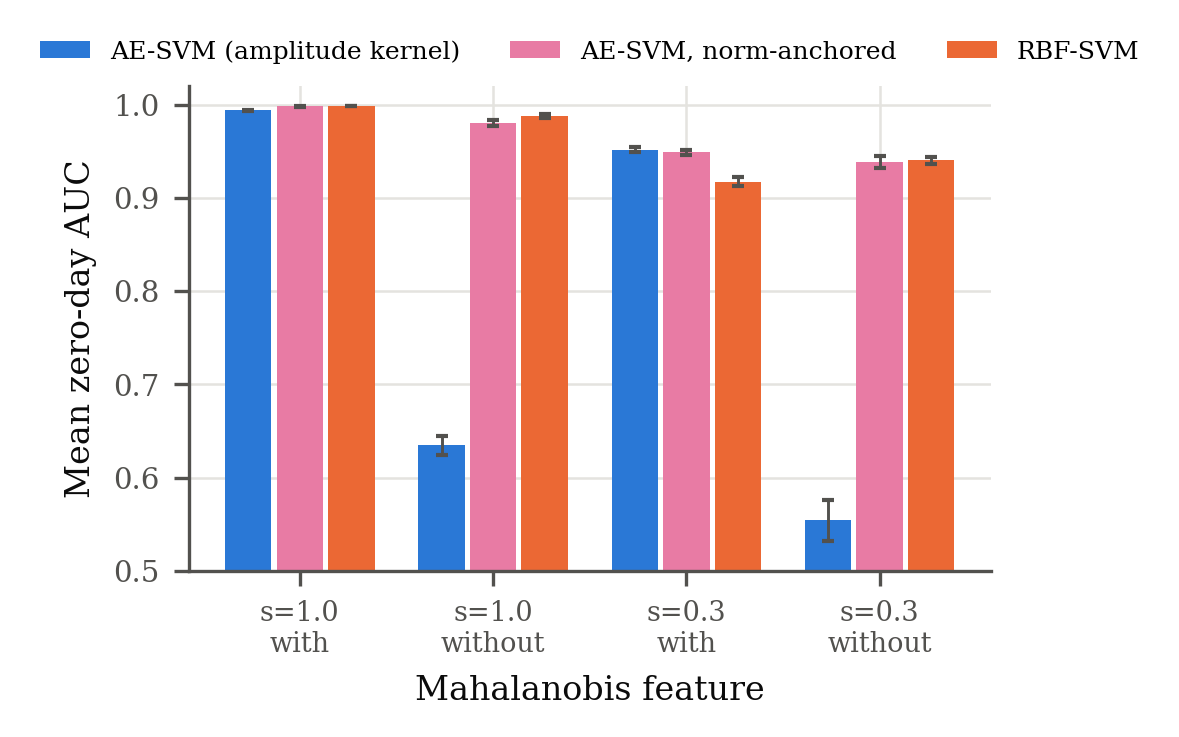
\includegraphics[width=0.92\columnwidth]{fig9_mahal_ablation.png}
  \caption{Mean zero-day AUC with and without the Mahalanobis feature. Without it, the amplitude kernel discards all magnitude information and fails on unseen attacks; a norm anchor restores it.}
  \label{fig:mahal}
\end{figure}

In leave-one-attack-out tests (Fig.~\ref{fig:zeroday}) AE-SVM generalizes as
well as RF and better than RBF-SVM at $s=0.3$ (mean AUC $0.952$ vs.\ $0.917$),
despite a lower kernel-target alignment~\cite{cristianini2002kernel}
with the labels ($0.13$--$0.22$ vs.\ $0.29$--$0.66$ across attack types). Proposition~\ref{prop:exact} suggests why
this is fragile: $K_A$ ignores $\|\mathbf{x}\|$, and an unseen attack is most
easily recognised by \emph{how far} it is from normal operation, which is a
magnitude. In our feature map that magnitude is carried by one coordinate, the
Mahalanobis distance. Removing it (Fig.~\ref{fig:mahal}) drops AE-SVM's mean
zero-day AUC to $0.554$ at $s=0.3$ and $0.635$ at $s=1$, while RBF-SVM is
unaffected ($0.940$, $0.987$). Appending a constant coordinate
$c=\mathrm{median}_{\mathrm{train}}\|\mathbf{x}\|$ before encoding, so that
$\phi(\mathbf{x})=(\mathbf{x},c)/\|(\mathbf{x},c)\|$ retains the input's norm relative
to $c$, restores AE-SVM to $0.939$ and $0.980$ without the Mahalanobis feature.

\subsection{When the amplitude kernel helps}

\begin{figure*}[t]
  \centering
  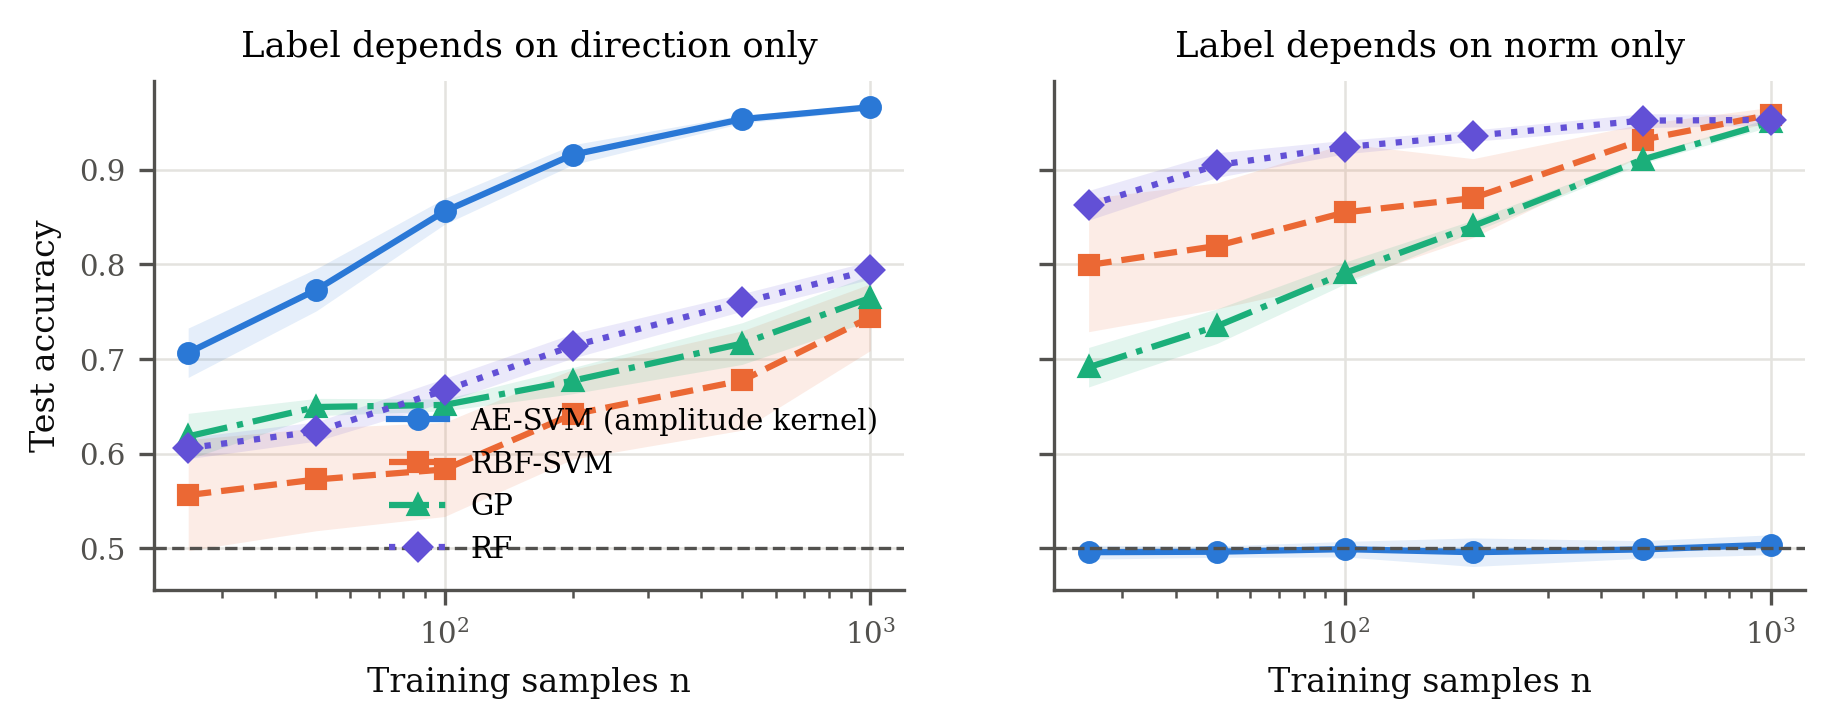
\includegraphics[width=0.92\textwidth]{fig8_kernel_crossover.png}
  \caption{Control tasks in $\mathbb{R}^8$ with heavy-tailed norms. Left: label depends on direction only. Right: label depends on norm only.}
  \label{fig:crossover}
\end{figure*}

Fig.~\ref{fig:crossover} isolates the inductive bias. When the label depends only
on direction and the norm is a heavy-tailed nuisance, AE-SVM learns from far
fewer samples than any baseline ($0.71$ vs.\ $0.56$ for RBF-SVM at $n=25$; $0.97$
vs.\ $0.74$ at $n=1000$). When the label depends only on norm, AE-SVM is at
chance at every $n$. QKD telemetry is neither extreme, which is why the kernel is
competitive but not superior on it.

\subsection{Calibration and selective prediction}
\label{sec:calib}

\begin{figure*}[t]
  \centering
  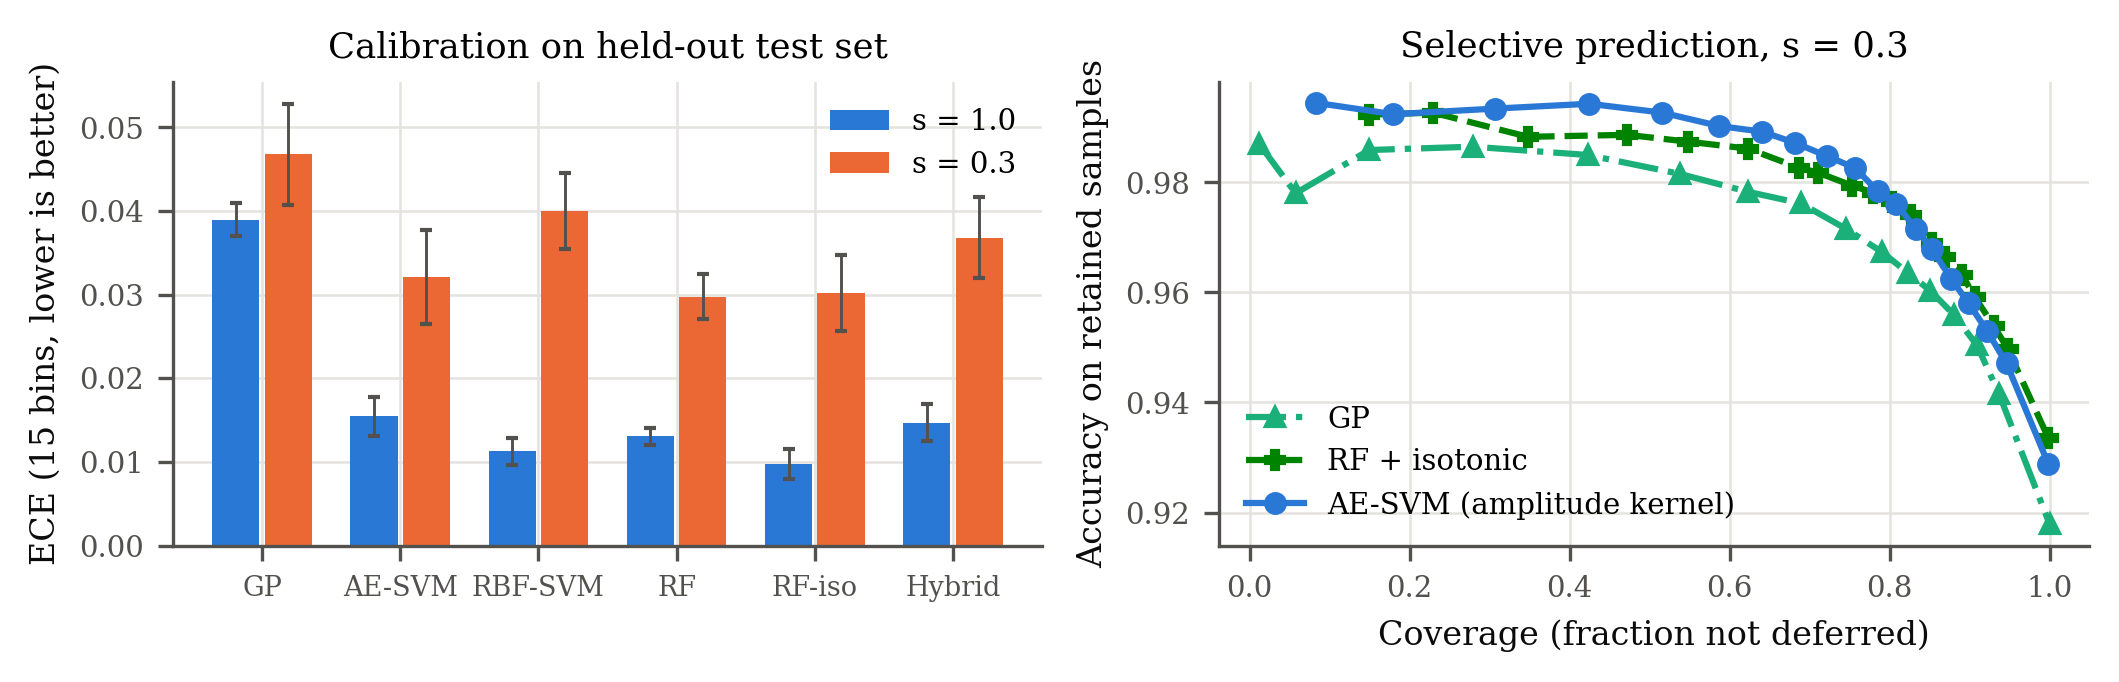
\includegraphics[width=0.92\textwidth]{fig6_calibration_selective.png}
  \caption{Left: ECE by model. Right: accuracy versus coverage when deferring samples with uncertainty $u=\sqrt{p(1-p)}$ above a threshold ($s=0.3$).}
  \label{fig:calib}
\end{figure*}

The GP's Laplace posterior is the least calibrated supervised model here
(ECE $0.047\pm0.006$ at $s=0.3$ and $0.039\pm0.002$ at $s=1$), and isotonic RF the
best ($0.030$ and $0.010$). For selective prediction (Fig.~\ref{fig:calib}), the
GP's probabilities are concentrated near the decision boundary: at threshold
$u<0.3$ it keeps $69\%$ of test blocks at $97.6\%$ accuracy, while isotonic RF
keeps $80\%$ at the same accuracy and AE-SVM $79\%$ at $97.8\%$; at $u<0.1$ the GP
retains no blocks at all at $s=0.3$. A model-based posterior is attractive in
principle, but on this data a cheaply recalibrated point estimator gives the
better deferral policy.

\subsection{Evasion and latency}

\begin{figure}[t]
  \centering
  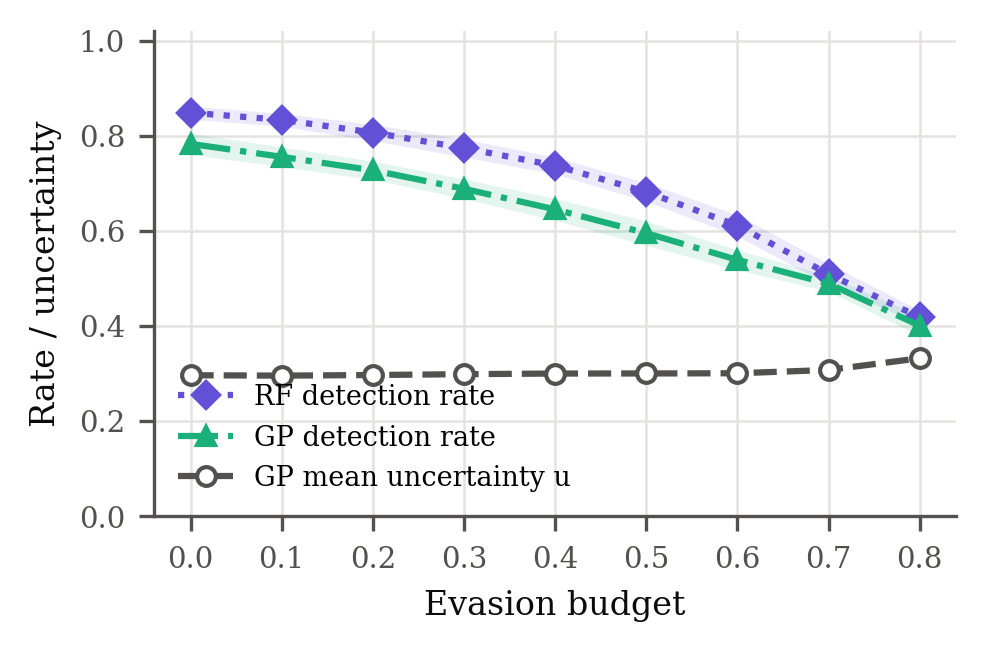
\includegraphics[width=\columnwidth]{fig7_adversarial.png}
  \caption{Detection rate of attack blocks ($s=0.3$) whose five most RF-important features are moved a fraction (the budget) of the way toward the normal median, and the GP's mean uncertainty on them.}
  \label{fig:adv}
\end{figure}

\begin{table}[t]
  \centering
  \caption{Inference latency on one CPU core (training excluded). Batch: amortised over 600 blocks. Single: median for one block, dominated by Python call overhead.}
  \label{tab:latency}
  \footnotesize
  \begin{tabular}{lrr}
    \toprule
    Component & Batch (ms/block) & Single (ms) \\
    \midrule
    Feature map & $0.0004$ & $0.14$ \\
    AE-SVM (exact) & $0.008$ & $0.35$ \\
    RBF-SVM & $0.012$ & $0.16$ \\
    RF (200 trees) & $0.093$ & $23.4$ \\
    Hybrid & $0.33$ & $26.9$ \\
    GP & $0.38$ & $29.6$ \\
    \bottomrule
  \end{tabular}
\end{table}

A simple gradient-free evasion that moves each attack block's five most
important features toward the normal median (Fig.~\ref{fig:adv}) lowers RF and
GP detection together, with RF ahead by 2--9 points at every budget at $s=0.3$
(2--10 points at $s=1$). The GP's
mean uncertainty on evading blocks barely changes ($0.30$ to $0.33$ at $s=0.3$),
so uncertainty alone does not flag this evasion. Table~\ref{tab:latency}
gives inference cost: all detectors are far below a per-block budget measured
in seconds; the kernel SVMs are cheapest in batch, and the GP and Hybrid models
are slowest.

\section{Limitations}
\label{sec:limits}

Every result is from simulation. The attack magnitudes are assumptions, and the
drift model, though grounded in standard channel physics, is not fitted to a
deployed link; the strength axis $s$ shows how conclusions move with signature
size but does not say which $s$ a real attacker produces. The evasion attack is
gradient-free and not adaptive. The detectors see per-block summaries only;
time-series models over consecutive blocks may do better. Validating the
ranking of methods, and the zero-day mechanism, on telemetry from a physical QKD
testbed is the necessary next step.

\section{Conclusion}
\label{sec:conclusion}

On a QKD telemetry simulator designed not to be trivially separable, random
forests are the strongest and most sample-efficient detector, isotonic
calibration gives better uncertainty for deferral than a GP posterior, and the
amplitude-encoding fidelity kernel---computable exactly on classical
hardware---is competitive but not superior. Its one distinctive behavior is
explained by Proposition~\ref{prop:exact}: it generalizes to unseen attacks only
when some feature carries the input's magnitude, and a norm anchor supplies that
when no such feature exists. Simulation-based QKD detection studies should
report single-feature separability and an attack-strength sweep alongside
headline accuracy.

\section*{Code and Data Availability}
Simulator, models, experiment driver (\texttt{scripts/hyqad/run\_experiments.py}),
figure script and every result CSV are at
\url{https://github.com/arnavk23/quasar-security}.

\bibliographystyle{IEEEtran}
\bibliography{../references}

\end{document}
